% !TeX program = lualatex
% Standalone plot: Chebyshev polynomials T_0, T_1, T_2, T_3 on [-1,1]

\documentclass[tikz, border=5pt]{standalone}
\usepackage{pgfplots}
\pgfplotsset{compat=newest}
\begin{document}
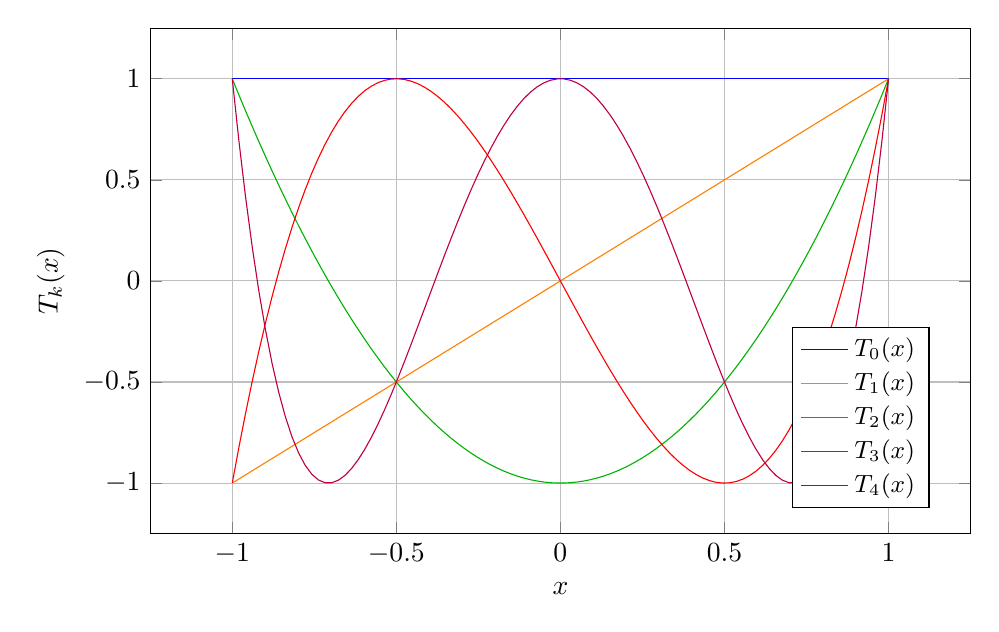
\begin{tikzpicture}
  \begin{axis}[
    width=12cm,
    height=8cm,
    xmin=-1.25, xmax=1.25,
    ymin=-1.25, ymax=1.25,
    xlabel={$x$}, ylabel={$T_k(x)$},
    xtick={-1,-0.5,0,0.5,1},
    ytick={-1,-0.5,0,0.5,1},
    grid=both,
    legend style={at={(0.95,0.05)}, anchor=south east, font=\small},
    legend cell align={left},
    samples=100
  ]
    % T_0(x) = 1
    \addplot[domain=-1:1, color=blue] {1};
    \addlegendentry{$T_0(x)$}
    % T_1(x) = x
    \addplot[domain=-1:1, color=orange] {x};
    \addlegendentry{$T_1(x)$}
    % T_2(x) = 2x^2 - 1
    \addplot[domain=-1:1, color=green!70!black] {2*x^2-1};
    \addlegendentry{$T_2(x)$}
    % T_3(x) = 4x^3 - 3x
    \addplot[domain=-1:1, color=red] {4*x^3-3*x};
    \addlegendentry{$T_3(x)$}
    % T_4(x) = 8x^4 - 8x^2 + 1
    \addplot[domain=-1:1, color=purple] {8*x^4-8*x^2+1};
    \addlegendentry{$T_4(x)$}
  \end{axis}
\end{tikzpicture}
\end{document}
